\documentclass[aspectratio=169, 10pt]{beamer}

% --- TEMA METROPOLIS E IMPOSTAZIONI ---
\usetheme{metropolis}
\usefonttheme{professionalfonts}
\metroset{
    numbering=fraction,
    progressbar=foot,
    block=transparent
}

% --- TIPOGRAFIA MODERNA E CONTROLLO SILLABAZIONE ---
\usepackage[T1]{fontenc}
\usepackage[utf8]{inputenc}
\usepackage[italian]{babel}
\usepackage[sfdefault]{FiraSans}
\usepackage[scaled=0.85]{beramono}
\usepackage[protrusion=true, expansion=false]{microtype}

% Controllo severo delle spezzature nei blocchi stretti
\tolerance=2000
\emergencystretch=2em
\hfuzz=1pt
\hyphenpenalty=8000
\exhyphenpenalty=8000

% --- MATEMATICA E SIMBOLI ---
\usepackage{amsmath, amssymb, amsfonts, mathtools}
\DeclareMathOperator{\atanTwo}{atan2}
\DeclareMathOperator{\sgn}{sgn}

% --- TABELLE E GRAFICA ---
\usepackage{booktabs}
\usepackage{array}
\usepackage{graphicx}
\graphicspath{{./Images/}}
\usepackage{tikz}
\usetikzlibrary{arrows.meta, positioning, shapes.geometric, calc}

% --- TCOLORBOX PER CARD MODERNE E TERMINALI ---
\usepackage[most]{tcolorbox}

% --- PALETTE COLORI (INGEGNERISTICA & ISTITUZIONALE) ---
\definecolor{UniPgNavy}{RGB}{15, 32, 54}        % Primario: Navy scuro profondo
\definecolor{TechCyan}{RGB}{0, 136, 160}        % Accento: Ciano industriale
\definecolor{AlertRed}{RGB}{195, 45, 45}        % Alert: Rosso vincoli/errori
\definecolor{SuccessGreen}{RGB}{38, 145, 80}    % Successo / Check
\definecolor{CardBg}{RGB}{248, 250, 252}        % Sfondo card chiare
\definecolor{CardBorder}{RGB}{215, 223, 233}    % Bordo delicato
\definecolor{TermBg}{RGB}{20, 23, 28}           % Sfondo terminale
\definecolor{TermBar}{RGB}{32, 36, 44}          % Barra mockup terminale

% --- COLORI METROPOLIS ---
\setbeamercolor{palette primary}{bg=UniPgNavy, fg=white}
\setbeamercolor{palette secondary}{bg=TechCyan, fg=white}
\setbeamercolor{progress bar}{fg=TechCyan, bg=gray!25}
\setbeamercolor{title separator}{fg=TechCyan}

% --- STILI CARD UNIFORMI (TCOLORBOX) ---
\tcbset{
    moderncard/.style={
        enhanced,
        colback=CardBg,
        colframe=CardBorder,
        boxrule=0.6pt,
        arc=3.5pt,
        boxsep=0pt,
        left=8pt,
        right=8pt,
        top=5pt,
        bottom=5pt,
        coltitle=UniPgNavy,
        fonttitle=\bfseries\footnotesize,
        attach title to upper=\par\vspace{2.5pt}
    },
    termframe/.style={
        enhanced,
        colback=TermBg,
        colframe=TermBar,
        boxrule=0.8pt,
        arc=4pt,
        boxsep=0pt,
        left=0pt,
        right=0pt,
        top=0pt,
        bottom=0pt,
        toptitle=3.5pt,
        bottomtitle=3.5pt,
        lefttitle=8pt,
        righttitle=8pt,
        title={%
            \tikz[baseline=-0.4ex]{
                \fill[red!85!black] (0, 0) circle (1.8pt);
                \fill[yellow!85!black] (5.5pt, 0) circle (1.8pt);
                \fill[green!80!black] (11pt, 0) circle (1.8pt);
            }%
            \hfill\fontsize{6.5pt}{7.5pt}\selectfont\texttt{\color{gray!50}terminal \textbullet{} bash}\hfill\hspace*{11pt}%
        },
        coltitle=white
    }
}

% --- MACRO PER FORMULE IN EVIDENZA ---
\newcommand{\formulaStrip}[1]{%
    \begin{tcolorbox}[
        enhanced, colback=UniPgNavy!6, colframe=UniPgNavy!20,
        boxrule=0.5pt, arc=3pt, boxsep=0pt,
        left=6pt, right=6pt, top=3.5pt, bottom=3.5pt,
        halign=center
    ]
        #1
    \end{tcolorbox}%
}

% --- METADATI ---
\title{Modellazione E Analisi Di Un Manipolatore RRP \mbox{(3 DoF)}}
\subtitle{Sviluppo di un Package ROS con Solutori Analitici e Controllo CLI}
\author[Francesco Lo Verde]{\textbf{Francesco Lo Verde}\texorpdfstring{\\[0.10cm]{\footnotesize\texttt{francesco.loverde@studenti.unipg.it}}}{}}
\institute{Università degli Studi di Perugia \quad---\quad Corso di Industrial Robotics}
\date{A.A. 2025 / 2026}

% ==============================================================================
\begin{document}

% AA SLIDE 1: FRONTESPIZIO
\begin{frame}[plain]
    \titlepage
\end{frame}

% AA SLIDE 2: INTRODUZIONE E OBIETTIVI
\begin{frame}{Obiettivi Ingegneristici del Progetto}
    \begin{columns}[onlytextwidth, T]
        \begin{column}{0.485\textwidth}
            \begin{tcolorbox}[moderncard, title={\color{UniPgNavy}Modellazione Parametrica}, equal height group=obj_top]
                \footnotesize
                \begin{itemize}
                    \setlength{\itemsep}{1.5pt}
                    \item Modello \textbf{XACRO / URDF} svincolato da quote cablate.
                    \item Caricamento dinamico dei link da configurazione \texttt{.yaml}.
                    \item Elevata modularità di montaggio su giunti standard.
                \end{itemize}
            \end{tcolorbox}

            \begin{tcolorbox}[moderncard, title={\color{TechCyan}Cinematica in Forma Chiusa}, equal height group=obj_bot]
                \footnotesize
                \begin{itemize}
                    \setlength{\itemsep}{1.5pt}
                    \item Risolutore Diretto: Convenzione \textbf{D-H Standard}.
                    \item Solutore Inverso analitico a tempo costante $\mathcal{O}(1)$.
                    \item Assoluta assenza di tolleranze o cicli iterativi.
                \end{itemize}
            \end{tcolorbox}
        \end{column}

        \begin{column}{0.485\textwidth}
            \begin{tcolorbox}[moderncard, title={\color{AlertRed}Controllo e Robustezza}, equal height group=obj_top]
                \footnotesize
                \begin{itemize}
                    \setlength{\itemsep}{1.5pt}
                    \item Verifica preventiva dello spazio $\mathcal{W}$ (\textit{clamping}).
                    \item Calcolo in tempo reale di singolarità via $\det(\mathbf{J}_p)$.
                    \item Scarto proattivo dei target non raggiungibili.
                \end{itemize}
            \end{tcolorbox}

            \begin{tcolorbox}[moderncard, title={\color{UniPgNavy}Architettura Software ROS}, equal height group=obj_bot]
                \footnotesize
                \begin{itemize}
                    \setlength{\itemsep}{1.5pt}
                    \item Doppia interfaccia: slider GUI e terminale CLI.
                    \item Parser simbolico avanzato tramite \textbf{SymPy}.
                    \item Ciclo a $20\text{ Hz}$ con filtro IIR di interpolazione d'uscita.
                \end{itemize}
            \end{tcolorbox}
        \end{column}
    \end{columns}
\end{frame}

% AA SLIDE 3: STRUTTURA MECCANICA E MODELLO URDF
\begin{frame}{Architettura Meccanica e Catena Cinematica}
    \begin{columns}[onlytextwidth, c]
        \begin{column}{0.60\textwidth}
            \begin{tcolorbox}[moderncard, title={\color{UniPgNavy}Specifiche dei Giunti e Dimensioni Meccaniche}]
                \footnotesize
                \begin{itemize}
                    \setlength{\itemsep}{2.5pt}
                    \item \textbf{Base Fissa:} blocco $0.30 \times 0.30 \times 0.05\text{ m}$;\\
                    offset globale $\mathbf{p}_{\text{base}} = [2.00, \; 0.00, \; 0.00]^T\text{ m}$.
                    \item \textbf{Giunto 1 (Rotoidale - Azimut):} rotazione asse $Z_0$;\\
                    escursione $q_1 \in [-\pi, +\pi]\text{ rad}$; colonna $l_1 = 0.55\text{ m}$.
                    \item \textbf{Giunto 2 (Rotoidale - Spalla):} rotazione asse $Y_1$;\\
                    limiti $q_2 \in [-\pi/2, +\pi/4]\text{ rad}$; braccio $l_2 = 0.45\text{ m}$.
                    \item \textbf{Giunto 3 (Prismatico - Stelo):} corsa $q_3 \in [0.00, 0.35]\text{ m}$;\\
                    scorrimento alloggiato nel box di guida terminale.
                    \item \textbf{End-Effector:} pinza a 2 dita rivolta verso il basso\\
                    (rotazione fissa $-180^\circ$ attorno all'asse $X$).
                \end{itemize}
            \end{tcolorbox}
        \end{column}

        \begin{column}{0.37\textwidth}
            \centering
            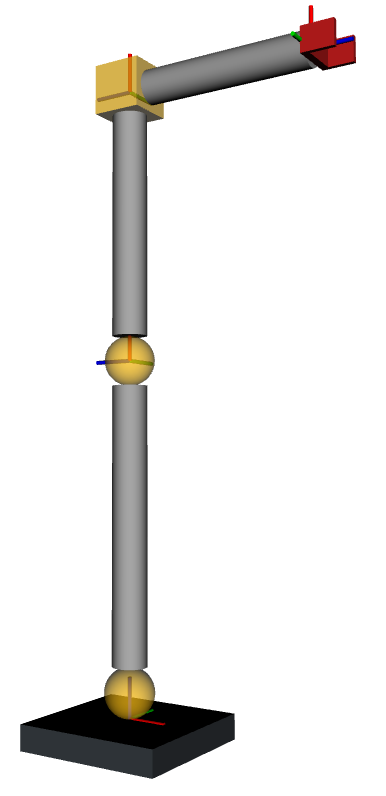
\includegraphics[height=0.70\textheight, keepaspectratio]{manipolatoreVerticale.png}
        \end{column}
    \end{columns}
\end{frame}

% AA SLIDE 4: CINEMATICA DIRETTA - TABELLA DH
\begin{frame}{Cinematica Diretta: Denavit-Hartenberg Standard}
    \vspace{-0.10cm}
    \formulaStrip{\small\color{UniPgNavy}
        $\mathbf{T}_{i-1}^i = \mathbf{R}_z(\theta_i) \, \mathbf{T}_z(d_i) \, \mathbf{T}_x(a_i) \, \mathbf{R}_x(\alpha_i)$
    }

    \vspace{0.10cm}
    \centering
    \renewcommand{\arraystretch}{1.18}
    {\footnotesize
    \begin{tabular}{lcccc}
        \toprule
        \textbf{Link} $i$ & $\boldsymbol{\theta_i}$ & $\mathbf{d_i}\text{ [m]}$ & $\mathbf{a_i}\text{ [m]}$ & $\boldsymbol{\alpha_i}\text{ [rad]}$ \\
        \midrule
        \textbf{1} ($RF_0 \to RF_1$) & $q_1$ & $d_1 = 2r_g + l_1 + r_g = 0.70$ & $0$ & $-\pi/2$ \\
        \textbf{2} ($RF_1 \to RF_2$) & $q_2$ & $0$ & $a_2 = r_g + l_2 + \tfrac{\text{box}}{2} = 0.55$ & $+\pi/2$ \\
        \textbf{3} ($RF_2 \to RF_{EE}$) & $0$ & $d_3 = q_3 - (l_3 + \tfrac{\text{box}}{2}) = q_3 - 0.40$ & $0$ & $-\pi$ \\
        \bottomrule
    \end{tabular}
    }

    \vspace{0.18cm}
    \begin{columns}[onlytextwidth, T]
        \begin{column}{0.485\textwidth}
            \begin{tcolorbox}[moderncard, title={\color{UniPgNavy}Parametri Geometrici di Offset}, equal height group=dh_bot]
                \footnotesize
                \begin{itemize}
                    \setlength{\itemsep}{1.5pt}
                    \item Raggio sfere dei giunti: $r_g = 0.05\text{ m}$
                    \item Lato box di raccordo: $\text{boxSize} = 0.10\text{ m}$
                    \item Corsa nominale stelo: $l_3 = 0.35\text{ m}$
                \end{itemize}
            \end{tcolorbox}
        \end{column}

        \begin{column}{0.485\textwidth}
            \begin{tcolorbox}[moderncard, title={\color{TechCyan}Escursione Variabile Link 3}, equal height group=dh_bot]
                \footnotesize
                \begin{itemize}
                    \setlength{\itemsep}{1.5pt}
                    \item Traslazione effettiva: $d_3 \in [-0.40, \; -0.05]\text{ m}$
                    \item Asse operativo: costantemente negativo
                    \item Assetto $\alpha_3 = -\pi \implies$ \mbox{gripper sempre verso terra}
                \end{itemize}
            \end{tcolorbox}
        \end{column}
    \end{columns}
\end{frame}

% AA SLIDE 5: CINEMATICA DIRETTA - POSA GLOBALE
\begin{frame}{Cinematica Diretta: Coordinate Cartesiane del TCP}
    \begin{columns}[onlytextwidth, c]
        \begin{column}{0.54\textwidth}
            \begin{tcolorbox}[moderncard, title={\color{UniPgNavy}Equazioni di Posizione del TCP}]
                \vspace{-0.15cm}
                \begin{align*}
                    X &= 2.00 + (a_2 \cos q_2 + d_3 \sin q_2) \cos q_1 \\
                    Y &= (a_2 \cos q_2 + d_3 \sin q_2) \sin q_1 \\
                    Z &= 0.05 + d_1 - a_2 \sin q_2 + d_3 \cos q_2
                \end{align*}
                \vspace{-0.22cm}
            \end{tcolorbox}

            \vspace{0.14cm}

            \begin{tcolorbox}[moderncard, title={\color{TechCyan}Configurazione di Home ($\mathbf{q} = [0, \; 0, \; 0]^T$)}]
                \footnotesize
                \begin{itemize}
                    \setlength{\itemsep}{2pt}
                    \item \textbf{Posizione TCP:} $\mathbf{p} = [2.55, \; 0.00, \; 0.35]^T\text{ m}$
                    \item \textbf{Assetto Finale:} $\mathbf{R} = \operatorname{diag}(1, -1, -1)$
                \end{itemize}
            \end{tcolorbox}
        \end{column}

        \begin{column}{0.43\textwidth}
            \centering
            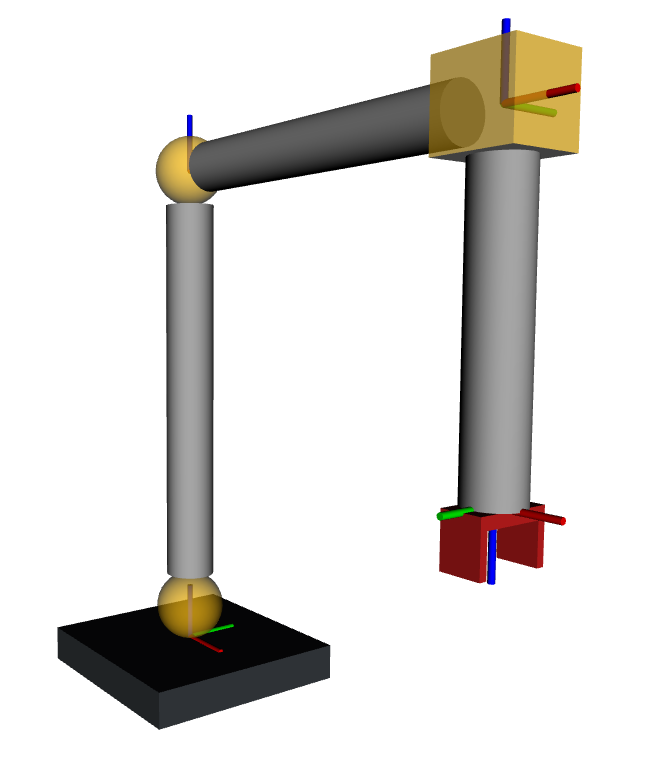
\includegraphics[width=\linewidth, keepaspectratio]{manipolatoreRRP.png}
        \end{column}
    \end{columns}
\end{frame}

% AA SLIDE 6: CINEMATICA INVERSA - q3 E q2
\begin{frame}{Cinematica Inversa: Risoluzione Analitica di $q_3$ e $q_2$}
    \vspace{-0.10cm}
    \formulaStrip{\footnotesize\color{UniPgNavy}
        Coordinate nel frame base $\{RF_0\}$: \quad $x = X - 2.00, \quad y = Y, \quad z = Z - 0.05$
    }

    \vspace{0.12cm}
    \begin{columns}[onlytextwidth, T]
        \begin{column}{0.485\textwidth}
            \begin{tcolorbox}[moderncard, title={\color{UniPgNavy}1. Giunto Prismatico ($q_3$)}, equal height group=ik_cards]
                \footnotesize
                Distanza radiale dalla spalla ($R_d^2$):
                \vspace{-0.08cm}
                \[
                    R_d^2 = x^2 + y^2 + (z - d_1)^2 = a_2^2 + d_3^2
                \]
                Risoluzione con $d_3 = q_3 - 0.40$:
                \vspace{-0.05cm}
                \[
                    \mathbf{q_3 = 0.40 - \sqrt{R_d^2 - a_2^2}}
                \]
                \textbf{Selezione fisica deterministica:}\\
                Il ramo col segno positivo implicherebbe \\
                $q_3 \ge 0.40\text{ m} > l_3$ (sfilamento fisico dello stelo).
            \end{tcolorbox}
        \end{column}

        \begin{column}{0.485\textwidth}
            \begin{tcolorbox}[moderncard, title={\color{TechCyan}2. Giunto di Spalla ($q_2$)}, equal height group=ik_cards]
                \footnotesize
                Posto il raggio piano $r = \sqrt{x^2 + y^2}$:
                \vspace{-0.08cm}
                \[
                    q_2 = \atanTwo(S_2, \, C_2)
                \]
                con $\begin{cases} S_2 = d_3 r - a_2(z - d_1) \\ C_2 = a_2 r + d_3(z - d_1) \end{cases}$

                \vspace{0.08cm}
                \textbf{Selezione di ramo deterministica:}\\
                Il ramo $-r$ richiederebbe angoli $q_2 < -90^\circ$ vietati dai finecorsa: si ammette solo il ramo frontale $+r$.
            \end{tcolorbox}
        \end{column}
    \end{columns}
\end{frame}

% AA SLIDE 7: CINEMATICA INVERSA - q1 E SINGOLARITÀ
\begin{frame}{Cinematica Inversa: Giunto $q_1$ e Robustezza}
    \begin{tcolorbox}[moderncard, title={\color{UniPgNavy}3. Giunto Azimutale di Base ($q_1$)}]
        \small
        Definendo il raggio proiettato orizzontale $\Delta = d_3 \sin q_2 + a_2 \cos q_2$, si ha $x = \Delta \cos q_1$, $y = \Delta \sin q_1$:
        \begin{itemize}
            \setlength{\itemsep}{2.5pt}
            \item \textbf{Gestione Singolarità sull'Asse ($|\Delta| < 10^{-6}\text{ m}$):}\\
            Il target giace esattamente sull'asse $Z_0$; l'azimut è ininfluente $\implies \mathbf{q_1 = 0.0\text{ rad}}$.
            \item \textbf{Soluzione Ordinaria in Forma Chiusa}:
            \[
                \mathbf{q_1 = \atanTwo\big(y \cdot \sgn(\Delta), \; x \cdot \sgn(\Delta)\big)}
            \]
        \end{itemize}
    \end{tcolorbox}

    \vspace{0.14cm}

    \begin{tcolorbox}[moderncard, title={\color{TechCyan}Determinismo e Stabilità Numerica $\mathcal{O}(1)$}]
        \small
        L'intero algoritmo opera a \textbf{tempo costante deterministico $\mathcal{O}(1)$}, senza richiedere inversioni di matrici Jacobiane né discese di gradiente.
        Questo garantisce l'azzeramento del jitter computazionale e l'assoluta assenza di divergenze numeriche.
    \end{tcolorbox}
\end{frame}

% AA SLIDE 8: SPAZIO DI LAVORO (WORKSPACE)
\begin{frame}{Analisi Geometrica dello Spazio di Lavoro (Workspace)}
    \begin{columns}[onlytextwidth, T]
        % --- COLONNA SINISTRA: TITOLO + IMMAGINE ---
        \begin{column}{0.48\textwidth}
            \centering
            % Blocco 1
            {\bfseries\footnotesize\color{UniPgNavy} Sezione Orizzontale (Vista X-Y)\par}
            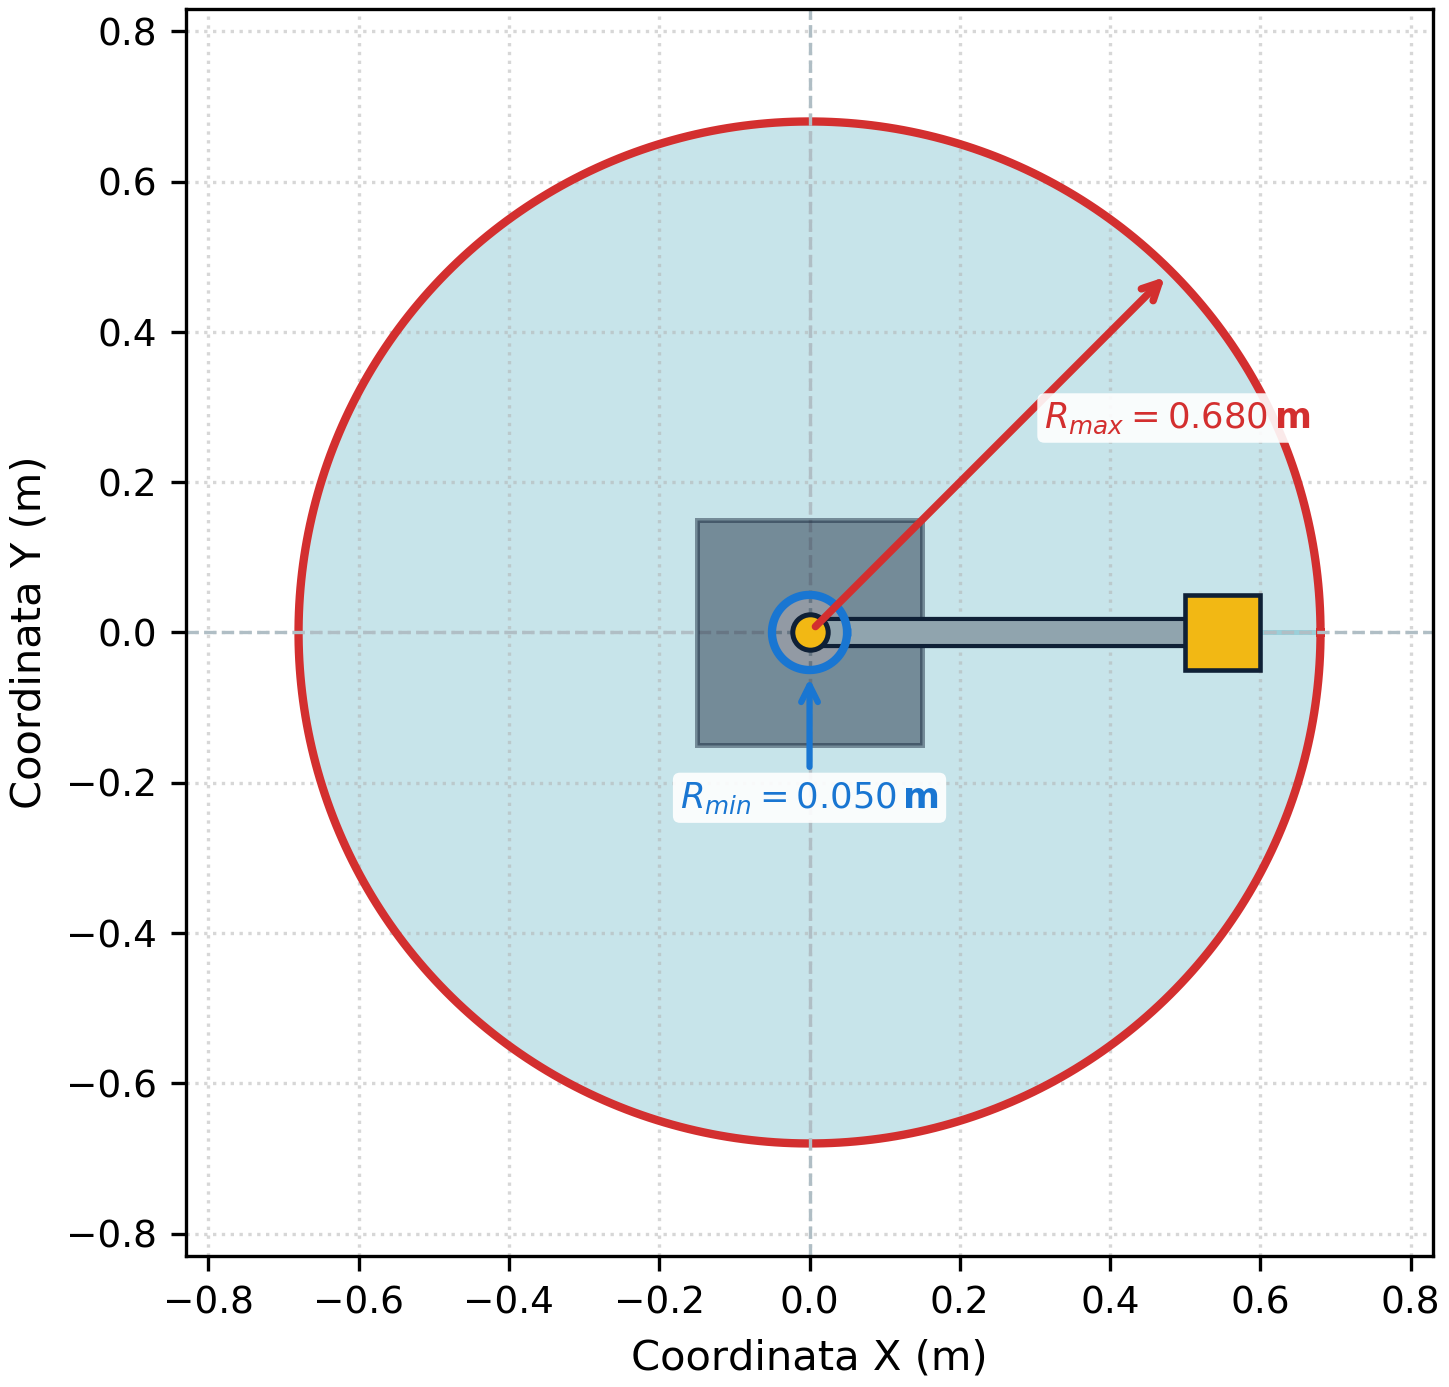
\includegraphics[width=\linewidth, height=0.43\textheight, keepaspectratio]{workspaceXYNoLegend.png}

            % Blocco 2
            {\bfseries\footnotesize\color{UniPgNavy} Sezione Verticale (Vista X-Z)\par}
            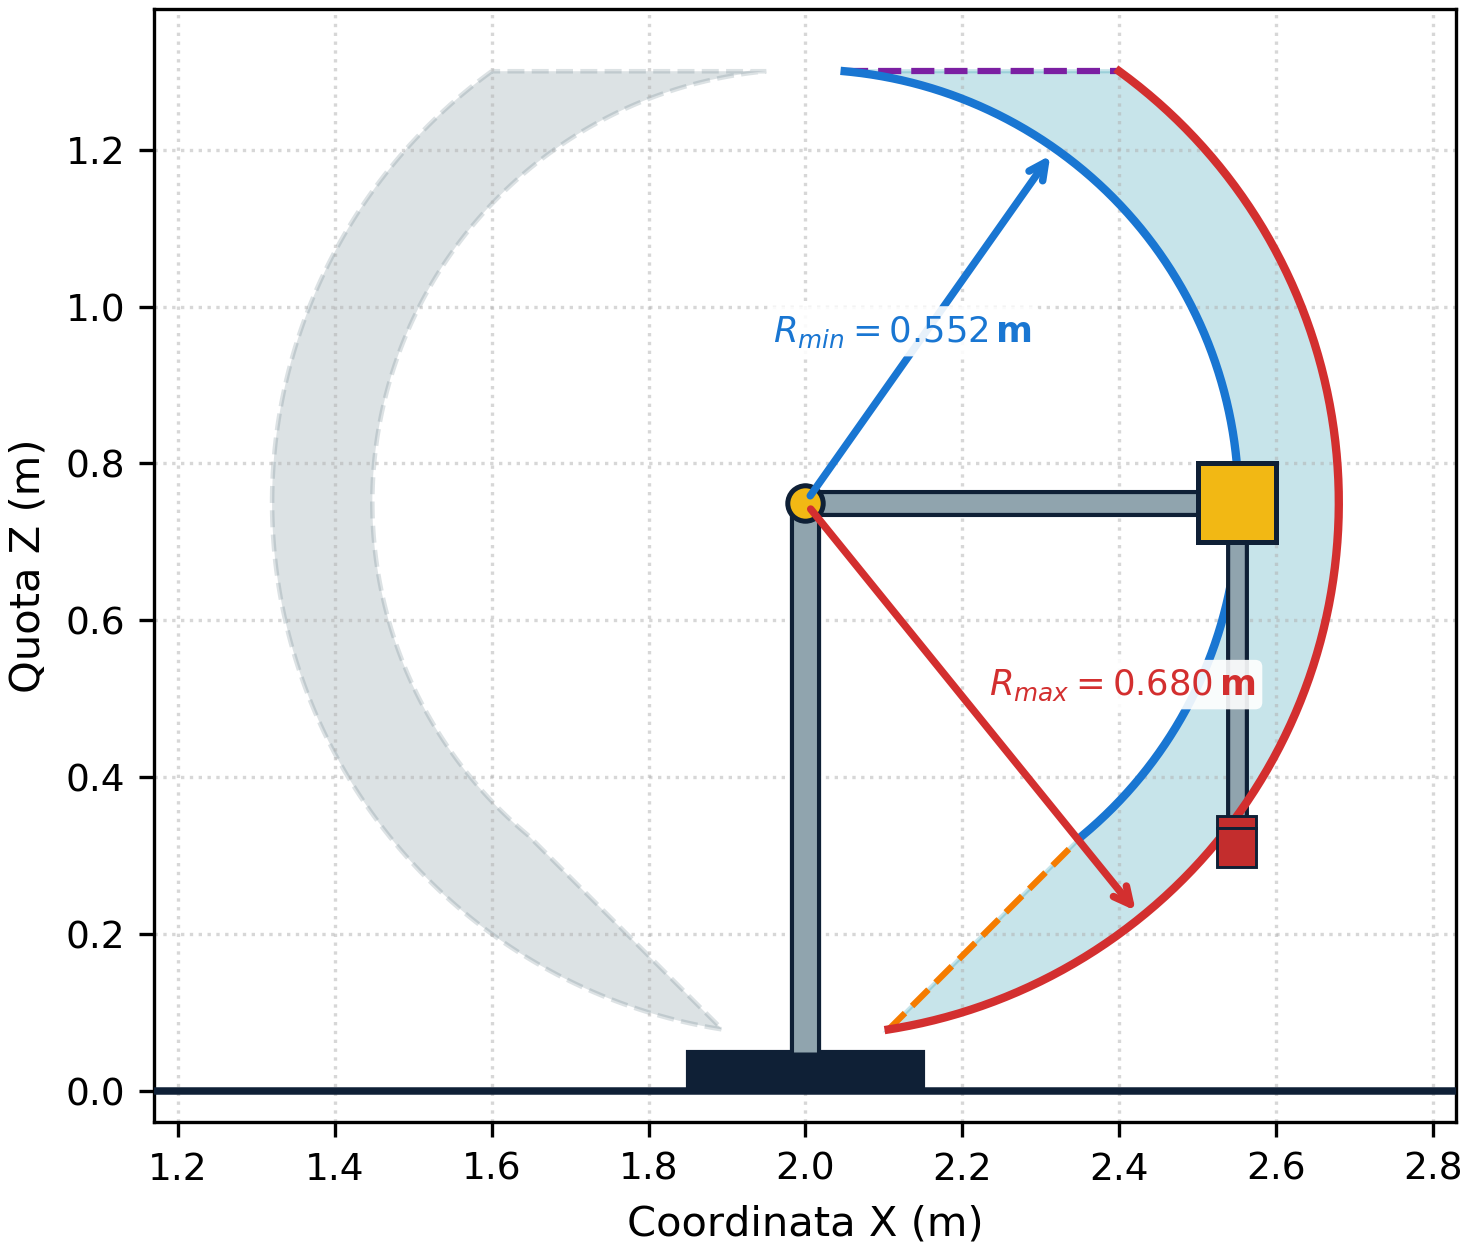
\includegraphics[width=\linewidth, height=0.43\textheight, keepaspectratio]{workspaceXZNoLegend.png}
        \end{column}

        % --- COLONNA DESTRA: LEGENDA + DIMENSIONI ---
        \begin{column}{0.50\textwidth}
            % CARD 1: LEGENDA CROMATICA
            \begin{tcolorbox}[moderncard,
                title={\color{UniPgNavy}Legenda Cromatica Unificata},
                top=2pt, bottom=2pt, left=3pt, right=3pt, boxsep=1pt,
                toptitle=1.5pt, bottomtitle=1.5pt]
                \fontsize{6.4pt}{8.0pt}\selectfont
                \begin{itemize}
                    \setlength{\itemsep}{1.2pt}
                    \setlength{\parskip}{0pt}
                    \setlength{\parsep}{0pt}
                    \setlength{\topsep}{0pt}
                    \setlength{\leftmargini}{1.1em}

                    \item[{\tikz[baseline=-0.5ex]\draw[red, line width=1.4pt] (0,0) -- (0.24,0);}]
                    \textbf{Raggio Max ($R_{\max} = 0.680\text{ m}$):} Sbraccio limite ($q_3 = 0$).

                    \item[{\tikz[baseline=-0.5ex]\draw[blue, line width=1.4pt] (0,0) -- (0.24,0);}]
                    \textbf{Raggio Min:}\enspace
                    \begin{tabular}[t]{@{}l@{}}
                        $R_{\min}^{XY} = 0.050\text{ m}$ \\
                        $R_{\min}^{XZ} = 0.552\text{ m}$ ($q_3 = l_3$).
                    \end{tabular}

                    \item[{\tikz[baseline=-0.5ex]\fill[TechCyan!35, draw=TechCyan, line width=0.5pt] (0,-0.04) rectangle (0.24,0.10);}]
                    \textbf{Area Raggiungibile:} Spazio frontale $\mathcal{W}$ ($q_1 = 0\text{ rad}$).

                    \item[{\tikz[baseline=-0.5ex]\draw[orange!90!black, line width=1.2pt, dashed] (0,0) -- (0.24,0);}]
                    \textbf{Limite Spalla Max:} Finecorsa $q_2 = +45^\circ$.

                    \item[{\tikz[baseline=-0.5ex]\draw[purple!80!black, line width=1.2pt, dashed] (0,0) -- (0.24,0);}]
                    \textbf{Limite Spalla Min:} Finecorsa $q_2 = -90^\circ$.

                    \item[{\tikz[baseline=-0.5ex]\fill[gray!25, draw=gray!70, dashed, line width=0.5pt] (0,-0.04) rectangle (0.24,0.10);}]
                    \textbf{Area Speculare:} Volume di rotazione $q_1 = \pm\pi\text{ rad}$.
                \end{itemize}
            \end{tcolorbox}

            \vspace{1.5mm}

            % CARD 2: DIMENSIONI E LIMITI OPERATIVI
            \begin{tcolorbox}[moderncard,
                title={\color{TechCyan}Dimensioni e Limiti Operativi},
                top=2pt, bottom=2pt, left=3pt, right=3pt, boxsep=1pt,
                toptitle=1.5pt, bottomtitle=1.5pt]
                \fontsize{6.4pt}{8.0pt}\selectfont
                \begin{itemize}
                    \setlength{\itemsep}{1.2pt}
                    \setlength{\parskip}{0pt}
                    \setlength{\parsep}{0pt}
                    \setlength{\topsep}{0pt}
                    \setlength{\leftmargini}{1.1em}

                    \item \textbf{Piano X-Y:} Toroide piano $0.050\text{ m} \le r \le 0.680\text{ m}$; azimut $q_1 \in [-\pi, +\pi]$ ($360^\circ$).
                    \item \textbf{Piano X-Z:} Settore sferico $0.552\text{ m} \le R_d \le 0.680\text{ m}$; spalla $q_2 \in [-90^\circ, +45^\circ]$ e corsa stelo $q_3 \in [0.00, 0.35]\text{ m}$.
                \end{itemize}
            \end{tcolorbox}
        \end{column}
    \end{columns}
\end{frame}

% AA SLIDE 9: ANALISI DIFFERENZIALE E JACOBIANO
\begin{frame}{Cinematica Differenziale e Analisi Jacobiana}
    \vspace{-0.10cm}
    \formulaStrip{\small\color{UniPgNavy}
        Mappatura differenziale: $\mathbf{v}_{TCP} = \mathbf{J}_p(\mathbf{q})\mathbf{\dot{q}}$ con $\mathbf{J}_p \in \mathbb{R}^{3 \times 3}$
    }

    \vspace{0.08cm}
    \begin{tcolorbox}[moderncard, title={\color{UniPgNavy}Determinante dello Jacobiano Posizionale}]
        \[
            \det(\mathbf{J}_p) = -d_3 \cdot [d_3 \sin(q_2) + a_2 \cos(q_2)]
        \]
        \centering\footnotesize\textit{Proprietà notevole:} $\det(\mathbf{J}_p)$ è rigorosamente indipendente dall'angolo azimutale $q_1$.
    \end{tcolorbox}

    \vspace{0.10cm}
    \begin{columns}[onlytextwidth, T]
        \begin{column}{0.485\textwidth}
            \begin{tcolorbox}[moderncard, title={\color{TechCyan}1. Singolarità Prismatica ($d_3 = 0$)}, equal height group=sing_cards]
                \footnotesize
                \textbf{Fisicamente Impossibile:}\\
                La corsa è limitata in $d_3 \in [-0.40, -0.05]\text{ m}$ \\in modo che il link non può collassare a zero.
            \end{tcolorbox}
        \end{column}

        \begin{column}{0.485\textwidth}
            \begin{tcolorbox}[moderncard, title={\color{TechCyan}2. Singolarità di Spalla ($\tan q_2 = -a_2 / d_3$)}, equal height group=sing_cards]
                \footnotesize
                \textbf{Preclusa dai Finecorsa:}\\
                Richiederebbe angoli $q_{2} \in [53.97^\circ, \; 84.81^\circ]$. \\ Il finecorsa meccanico del braccio è bloccato \\a $+45^\circ$.
            \end{tcolorbox}
        \end{column}
    \end{columns}
\end{frame}

% AA SLIDE 10: ARCHITETTURA SOFTWARE ROS E TF2
\begin{frame}{Architettura Software ROS e Albero TF2}
    \begin{columns}[onlytextwidth, T]
        % --- COLONNA SINISTRA: GRAFI COMPUTAZIONALI ---
        \begin{column}{0.54\textwidth}
            \begin{tcolorbox}[moderncard, title={\color{UniPgNavy}Modalità GUI (\texttt{gui:=true})}]
                \centering
                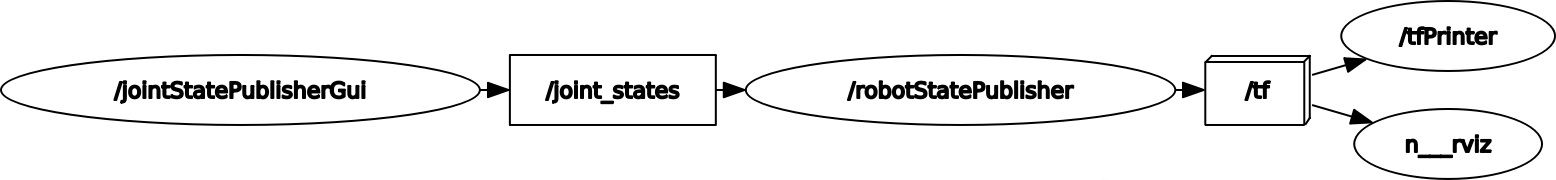
\includegraphics[width=\linewidth, keepaspectratio]{rqtGraphWithGUI.png}
            \end{tcolorbox}

            \vspace{0.10cm}

            \begin{tcolorbox}[moderncard, title={\color{TechCyan}Modalità CLI Interattiva (\texttt{gui:=false})}]
                \centering
                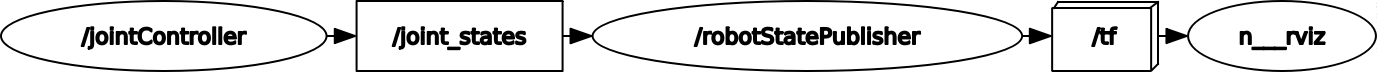
\includegraphics[width=\linewidth, keepaspectratio]{rqtGraphNoGUI.png}
            \end{tcolorbox}
        \end{column}

        % --- COLONNA DESTRA: ALBERO TF ---
        \begin{column}{0.43\textwidth}
            \begin{tcolorbox}[moderncard, title={\color{UniPgNavy}Albero delle Trasformate (\texttt{tf2})}]
                \centering
                \vspace{0.05cm}
                \tikzset{
                    tfNode/.style={
                        rectangle, rounded corners=2.5pt,
                        draw=UniPgNavy!70, line width=0.7pt, fill=white,
                        text=UniPgNavy, font=\fontsize{7pt}{8pt}\selectfont\bfseries,
                        minimum width=2.15cm, minimum height=0.38cm,
                        align=center
                    },
                    tfRoot/.style={tfNode, draw=UniPgNavy, fill=UniPgNavy, text=white},
                    tfEE/.style={tfNode, draw=AlertRed, fill=AlertRed!10, text=AlertRed!90!black},
                    tagStat/.style={fill=gray!20, text=gray!80!black, font=\fontsize{5.2pt}{5.8pt}\selectfont, rounded corners=2pt, inner sep=1.8pt},
                    tagDyn/.style={fill=TechCyan!15, text=TechCyan!90!black, font=\fontsize{5.4pt}{6.0pt}\selectfont\bfseries, rounded corners=2pt, inner sep=1.8pt},
                    tfLink/.style={-{Stealth[length=4pt, width=2.8pt]}, draw=UniPgNavy!70, line width=0.8pt}
                }

                % Distanza tra nodi incrementata a 0.48cm per frecce visibilmente più lunghe e ariose
                \begin{tikzpicture}[node distance=0.48cm]
                    \node[tfRoot]                 (world) {\texttt{world}};
                    \node[tfNode, below=of world] (base)  {\texttt{base}};
                    \node[tfNode, below=of base]  (rf0)   {\texttt{RF0}};
                    \node[tfNode, below=of rf0]   (rf1)   {\texttt{RF1}};
                    \node[tfNode, below=of rf1]   (rf2)   {\texttt{RF2}};
                    \node[tfEE,   below=of rf2]   (ee)    {\texttt{endEffector}};

                    \draw[tfLink] (world) -- node[right=0.08cm, tagStat] {Static ($X = +2.0\text{ m}$)} (base);
                    \draw[tfLink] (base)  -- node[right=0.08cm, tagDyn]  {Giunto 1 ($q_1$)} (rf0);
                    \draw[tfLink] (rf0)   -- node[right=0.08cm, tagDyn]  {Giunto 2 ($q_2$)} (rf1);
                    \draw[tfLink] (rf1)   -- node[right=0.08cm, tagDyn]  {Giunto 3 ($q_3$)} (rf2);
                    \draw[tfLink] (rf2)   -- node[right=0.08cm, tagStat] {Static (Pinza)} (ee);
                \end{tikzpicture}

                \vspace{0.08cm}
                {\fontsize{5.8pt}{6.8pt}\selectfont\color{gray!70!black} Broadcast a $20\text{ Hz}$ (\texttt{robot\_state\_publisher})}
            \end{tcolorbox}
        \end{column}
    \end{columns}
\end{frame}

% AA SLIDE 11: NODO CLI E CINEMATICA DIRETTA
\begin{frame}{Nodo di Controllo CLI ed Esecuzione Diretta}
    \begin{columns}[onlytextwidth, c]
        \begin{column}{0.485\textwidth}
            \begin{tcolorbox}[moderncard, title={\color{UniPgNavy}Parser Simbolico (SymPy)}]
                \footnotesize
                Supporto nativo a espressioni matematiche ed angoli simbolici (es.~\texttt{pi/4}, \texttt{pi/7}, frazioni).
            \end{tcolorbox}

            \vspace{0.12cm}

            \begin{tcolorbox}[moderncard, title={\color{TechCyan}Filtro IIR di Interpolazione}]
                \footnotesize
                Filtro digitale passa-basso ($\alpha = 0.15$ a $20\text{ Hz}$) per garantire movimenti morbidi ed eliminare scatti.
            \end{tcolorbox}

            \vspace{0.12cm}

            \begin{tcolorbox}[moderncard, title={\color{TechCyan}Monitor di Sicurezza in Linea}]
                \footnotesize
                Verifica del determinante in tempo reale:\\
                $\det(\mathbf{J}_p) = 0.081751 \implies \text{\textbf{\color{SuccessGreen}[Sicuro]}}$.
            \end{tcolorbox}
        \end{column}

        \begin{column}{0.485\textwidth}
            \begin{tcolorbox}[termframe]
                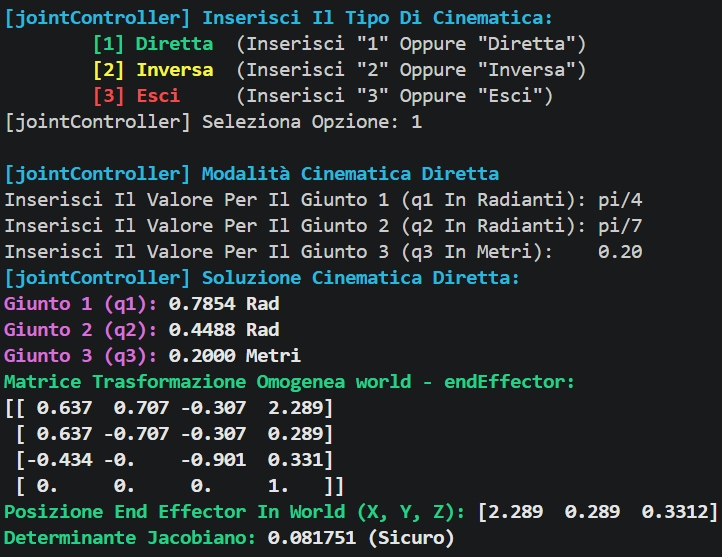
\includegraphics[width=\linewidth, keepaspectratio]{cinematicaDirettaCLI.png}
            \end{tcolorbox}
        \end{column}
    \end{columns}
\end{frame}

% AA SLIDE 12: ROBUSTEZZA E CONTROLLO LIMITI
\begin{frame}{Validazione Sperimentale e Sicurezza Operativa}
    \begin{columns}[onlytextwidth, c]
        \begin{column}{0.485\textwidth}
            \begin{tcolorbox}[moderncard, title={\color{UniPgNavy}Controllo Difensivo \texttt{checkWorkspace}}]
                \footnotesize
                Distanza radiale calcolata rispetto alla spalla:
                \vspace{-0.08cm}
                \[
                    d = \sqrt{(X - 2.0)^2 + Y^2 + (Z - 0.75)^2}
                \]
                \vspace{-0.15cm}
                \centering
                \textbf{Range ammesso:} $0.5523\text{ m} \le d \le 0.6801\text{ m}$
            \end{tcolorbox}

            \vspace{0.075cm}

            \begin{tcolorbox}[moderncard, title={\color{AlertRed}Intercettazione Target Fuori Limite}]
                \footnotesize
                \textbf{Target Cartesiano Inserito:}\\
                $\mathbf{p}_{\text{cmd}} = [2.40, 0.70, 0.10]^T\text{ m} \rightarrow d = 1.0356\text{ m}$

                \vspace{0.06cm}
                $d = 1.0356 > 0.6801\text{ m} \rightarrow$ \textbf{Non Raggiungibile}
            \end{tcolorbox}
        \end{column}

        \begin{column}{0.485\textwidth}
            \begin{tcolorbox}[termframe]
                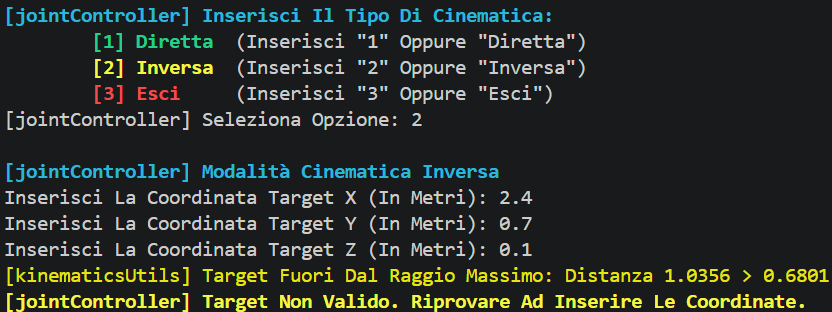
\includegraphics[width=\linewidth, keepaspectratio]{workspaceErrorCLI.png}
            \end{tcolorbox}

            \vspace{0.075cm}

            \begin{tcolorbox}[moderncard, title={\color{SuccessGreen}Integrità Cinematica Preservata}]
                \footnotesize
                L'architettura garantisce l'immunità da collisioni interne ed esclude setpoint non conformi al generatore.
            \end{tcolorbox}
        \end{column}
    \end{columns}
\end{frame}

% AA SLIDE 13: CONCLUSIONI E SVILUPPI FUTURI
\begin{frame}{Conclusioni e Sviluppi Futuri}
    \begin{columns}[onlytextwidth, T]
        \begin{column}{0.485\textwidth}
            \begin{tcolorbox}[moderncard, title={\color{UniPgNavy}Sintesi dei Risultati}, equal height group=concl_cards]
                \footnotesize
                \begin{itemize}
                    \setlength{\itemsep}{2.5pt}
                    \item \textbf{Modello URDF / XACRO Parametrico:}\\
                    Quote geometriche centralizzate su \texttt{.yaml} per facilitare riconfigurazioni strutturali.
                    \item \textbf{Simulazione RViz e Controllo Duale:}\\
                    Interfaccia condizionale flessibile: slider grafici (GUI) oppure terminale interattivo (CLI).
                    \item \textbf{Suite Cinematica Analitica $\mathcal{O}(1)$:}\\
                    Solutori chiusi per cinematica diretta, inversa e determinante Jacobiano senza iterazioni.
                    \item \textbf{Validazione e Sicurezza Operativa:}\\
                    Coerenza confermata su albero \texttt{tf2}; blocco difensivo preventivo fuori workspace.
                \end{itemize}
            \end{tcolorbox}
        \end{column}

        \begin{column}{0.485\textwidth}
            \begin{tcolorbox}[moderncard, title={\color{TechCyan}Prospettive di Sviluppo Futuro}, equal height group=concl_cards]
                \footnotesize
                \begin{itemize}
                    \setlength{\itemsep}{3.5pt}
                    \item \textbf{Pianificazione e Traiettorie:}\\
                    Generazione del moto nello spazio dei giunti con continuità di velocità e accelerazione, minimizzando le sollecitazioni dinamiche.
                    \item \textbf{Simulazione Dinamica in Gazebo:}\\
                    Estensione oltre la geometria: integrazione delle equazioni della dinamica, forze esterne e regolatori industriali di coppia ad anello chiuso.
                \end{itemize}
            \end{tcolorbox}
        \end{column}
    \end{columns}
\end{frame}

\end{document}
